\documentclass[10pt]{article}
\usepackage{itcep, stmaryrd, tikz, pgflibraryplotmarks, multicol, pgfplots}
\usepackage[margin=1in, nohead, pdftex]{geometry}

\topmargin -0.2in
\pagestyle{empty}
\singlespacing
\let\oldhat\hat
\renewcommand{\vec}[1]{\mathbf{#1}}
\renewcommand{\hat}[1]{\oldhat{\mathbf{#1}}}

\definecolor{light-gray}{gray}{0.95}
\newcommand{\code}[1]{\colorbox{light-gray}{\texttt{#1}}}

\newcommand{\headerclass}{Machine Learning Camp}
\newcommand{\headersection}{Day 2: Introduction to Classification}
\newcommand{\headertitle}{Won't you be my neighbor?}

\def\C{\mathbb{C}}
\def\R{\mathbb{R}}
\parindent 0ex
\begin{document}
%==================================================================================================================================================
\headerclass\xspace \hspace{\stretch{1}} \headersection\\
\begin{center}{ \large \textbf{\headertitle} }\end{center}
%==================================================================================================================================================

There are a lot of different algorithms which can be used to classify data. The first one that we'll cover is called the \emph{$k$-nearest neighbors} algorithm. For this algorithm,
\begin{enumerate}
\item We pick a number $k$.
\item In order to classify a point $P$, we look at the $k$ data points which are closest to $P$. 
\item These $k$ data points ``vote'' on what they think $P$ should be, and the majority wins.
\end{enumerate}

We'll practice this with an example.

\begin{center}
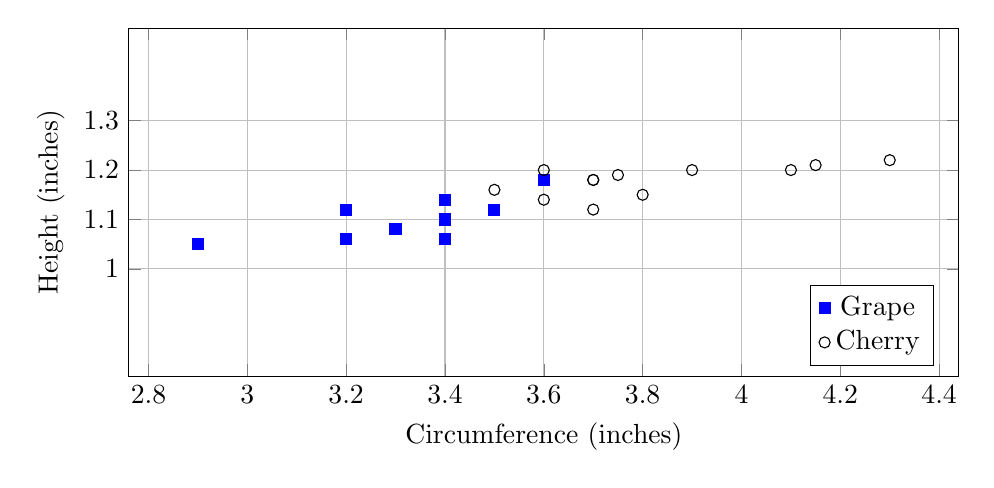
\begin{tikzpicture}
\begin{axis}[grid=both,
	legend pos=south east,
    xlabel= {Circumference (inches)},
    ylabel= {Height (inches)},
    width = \textwidth,
    height = 6cm,
    ytick={1,1.1,1.2,1.3},
    axis equal
  ]
    \addplot[
        scatter,only marks,scatter src=explicit symbolic,
        scatter/classes={
            a={mark=square*,blue},
            b={mark=o,draw=black,fill=black}
        }
    ]
    table[x=x,y=y,meta=label]{
        y    x    label
        1.18 3.7 b
        1.06 3.2 a
        1.08 3.3 a
        1.06 3.4 a
        1.05 2.9 a
        1.12 3.5 a
        1.14 3.4 a
        1.18 3.6 a
        1.18 3.7 b
        1.16 3.5 b
        1.14 3.6 b
        1.12 3.7 b
        1.19 3.75 b
        1.20 3.9 b
        1.20 3.6 b
        1.22 4.3 b
        1.20 4.1 b
        1.21 4.15 b
        1.15 3.8 b
        1.1 3.4 a
        1.12 3.2 a

    };
    \legend{Grape, Cherry}
\end{axis}
\end{tikzpicture}
\end{center}

For our example, we'll work with $k=3$. So, for a new point $P$, we'll use the $3$ closest data point to classify that point.

\begin{enumerate}

\item Plot the point $P$ for a fruit with circumference 4 inches and height 1.2 inches. Which $3$ data points are closest to $P$? Are they grapes or cherries?
\vspace{1.5cm}

Based on those three neighbors, would we classify $P$ as a grape or a cherry?
\vspace{1cm}

\item Plot the point $Q$ for a fruit with circumference 3.6 inches and height 1.16 inches. Which $3$ data points are closest to $Q$? Are they grapes or cherries?
\vspace{1.5cm}

Based on those three neighbors, would we classify $Q$ as a grape or a cherry?
\vspace{1cm}

\vfill
\item Shade in the region of your graph that would be classified as cherries using the $3$-nearest neighbors algorithm.

\newpage

\item Suppose instead of using the $3$ nearest neighbors, we took $k=1$ and only used the single closest data point. Shade in the region of the graph that would be classified as cherries using the $1$-nearest neighbors algorithm.

\begin{center}
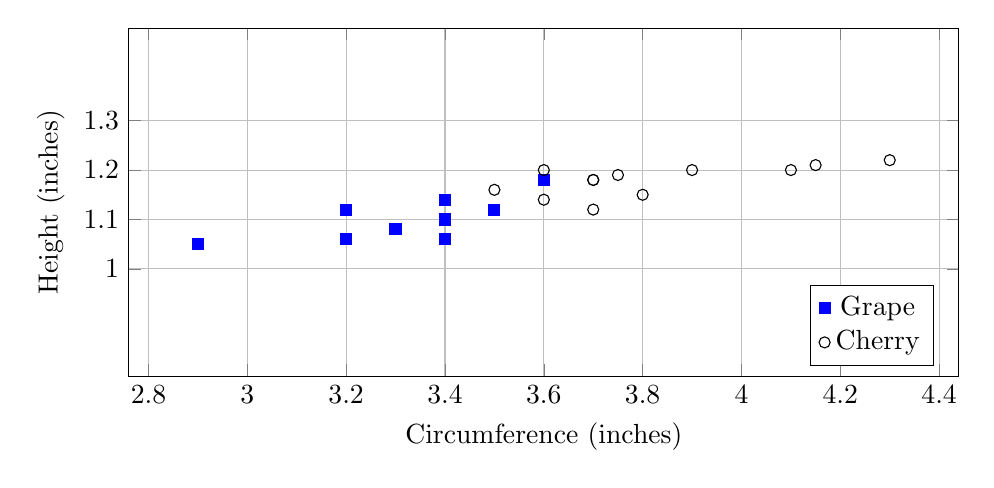
\begin{tikzpicture}
\begin{axis}[grid=both,
	legend pos=south east,
    xlabel= {Circumference (inches)},
    ylabel= {Height (inches)},
    width = \textwidth,
    height = 6cm,
    ytick={1,1.1,1.2,1.3},
    axis equal
  ]
    \addplot[
        scatter,only marks,scatter src=explicit symbolic,
        scatter/classes={
            a={mark=square*,blue},
            b={mark=o,draw=black,fill=black}
        }
    ]
    table[x=x,y=y,meta=label]{
        y    x    label
        1.18 3.7 b
        1.06 3.2 a
        1.08 3.3 a
        1.06 3.4 a
        1.05 2.9 a
        1.12 3.5 a
        1.14 3.4 a
        1.18 3.6 a
        1.18 3.7 b
        1.16 3.5 b
        1.14 3.6 b
        1.12 3.7 b
        1.19 3.75 b
        1.20 3.9 b
        1.20 3.6 b
        1.22 4.3 b
        1.20 4.1 b
        1.21 4.15 b
        1.15 3.8 b
        1.1 3.4 a
        1.12 3.2 a

    };
    \legend{Grape, Cherry}
\end{axis}
\end{tikzpicture}
\end{center}

Do you think the $1$-nearest neighbor classification is better or worse than the $3$-nearest neighbor classification? Why?
\vfill

\item Suppose instead of using the $3$ nearest neighbors, we took $k=20$ and used the $20$ closest data points. Shade in the region of the graph that would be classified as cherries using the $20$-nearest neighbors algorithm.

\begin{center}
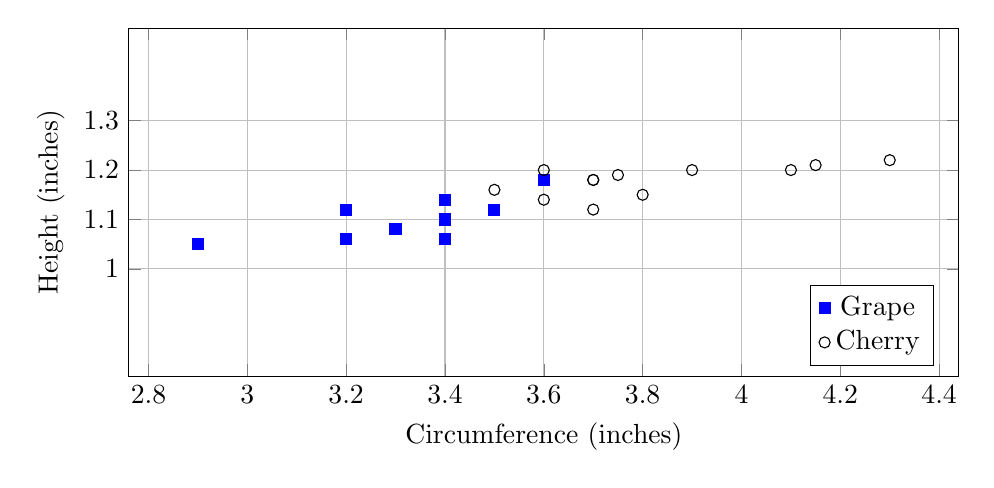
\begin{tikzpicture}
\begin{axis}[grid=both,
	legend pos=south east,
    xlabel= {Circumference (inches)},
    ylabel= {Height (inches)},
    width = \textwidth,
    height = 6cm,
    ytick={1,1.1,1.2,1.3},
    axis equal
  ]
    \addplot[
        scatter,only marks,scatter src=explicit symbolic,
        scatter/classes={
            a={mark=square*,blue},
            b={mark=o,draw=black,fill=black}
        }
    ]
    table[x=x,y=y,meta=label]{
        y    x    label
        1.18 3.7 b
        1.06 3.2 a
        1.08 3.3 a
        1.06 3.4 a
        1.05 2.9 a
        1.12 3.5 a
        1.14 3.4 a
        1.18 3.6 a
        1.18 3.7 b
        1.16 3.5 b
        1.14 3.6 b
        1.12 3.7 b
        1.19 3.75 b
        1.20 3.9 b
        1.20 3.6 b
        1.22 4.3 b
        1.20 4.1 b
        1.21 4.15 b
        1.15 3.8 b
        1.1 3.4 a
        1.12 3.2 a

    };
    \legend{Grape, Cherry}
\end{axis}
\end{tikzpicture}
\end{center}

Do you think the $20$-nearest neighbor classification is better or worse than the $3$-nearest neighbor classification? Why?
\vfill

How can you decide what value of $k$ works well for $k$-nearest neighbor classification?
\end{enumerate}



\end{document}
